\chapter{Leçon 24: Genren, Artikelen an Diminutiven}

Dës Lektioun erkläert d'Reegelen iwwert de Genre vun den Nimm, d'Artikelen am Nominativ an Akkusativ, an d'Diminutiven. \textit{Cette leçon explique les règles sur le genre des noms, les articles au nominatif et accusatif, et les diminutifs. / This lesson explains the rules on noun genders, articles in the nominative and accusative, and diminutives.}

\vspace{1em}

\section[Den Artikel / L'Article / The Article]{Den Artikel (Nominativ, Akkusativ) \\/ L'article (Nominatif, Accusatif) \\/ The Article (Nominative, Accusative)}

Am Lëtzebuergesche sinn den Nominativ an den Akkusativ fir d'Artikelen formell identesch. \textit{En luxembourgeois, le nominatif et l'accusatif sont formellement identiques pour les articles. / In Luxembourgish, the nominative and accusative are formally identical for articles.}

\vspace{0.5em}

\begin{tabular}{lllll}
    \toprule
    \textbf{Artikel / Article} & \textbf{Männlech (m)} & \textbf{Weiblech (w)} & \textbf{Sächlech (s)} & \textbf{Plural (pl)} \\
    \midrule
    \textbf{onbestëmmt} \textit{(indéfini / indefinite)} & e(n) & eng & e(n) & / \\
    \textbf{bestëmmt} \textit{(défini / definite)} & de(n) & d' & d' & d' \\
    \bottomrule
\end{tabular}

\vspace{1em}

\textbf{Bemierkungen / Remarques / Notes:}
\begin{itemize}
    \item Ob \textbf{e} oder \textbf{en} (onbestëmmt) a \textbf{de} oder \textbf{den} (bestëmmt) benotzt gëtt, hänkt vun der \textbf{n-Reegel} (Eifeler Regel) of. De finalen \textit{-n} bleift virun Vokalen (a, e, i, o, u) an de Konsonanten d, t, n, h, z, souwéi virun Interpunktiounszeechen.
    \item \textit{La règle de l'Eifeler Regel s'applique pour le masculin et le neutre. Le -n final est conservé devant les voyelles et les consonnes d, t, n, h, z. / The Eifeler Regel rule applies for masculine and neuter. The final -n is kept before vowels and the consonants d, t, n, h, z.}
\end{itemize}

\vspace{0.5em}
\textbf{Beispiller / Exemples / Examples:}
\begin{itemize}
    \item \textbf{Männlech:} Dat ass \textbf{en} Auto. $\rightarrow$ Dat ass \textbf{den} Auto. \textit{(C'est une voiture. $\rightarrow$ C'est la voiture. / That is a car. $\rightarrow$ That is the car.)}
    \item \textbf{Weiblech:} Dat ass \textbf{eng} Camionnette. $\rightarrow$ Dat ass \textbf{d'}Camionnette. \textit{(C'est une camionnette. $\rightarrow$ C'est la camionnette. / That is a van. $\rightarrow$ That is the van.)}
    \item \textbf{Sächlech:} Dat ass \textbf{e} Boot. $\rightarrow$ Dat ass \textbf{d'}Boot. \textit{(C'est un bateau. $\rightarrow$ C'est le bateau. / That is a boat. $\rightarrow$ That is the boat.)}
    \item \textbf{Plural:} Dat si(nn) Autoen. $\rightarrow$ Dat si(nn) \textbf{d'}Autoen. \textit{(Ce sont des voitures. $\rightarrow$ Ce sont les voitures. / Those are cars. $\rightarrow$ Those are the cars.)}
\end{itemize}

\vspace{1cm}

\section[Genre-Reegelen / Règles de Genre / Gender Rules]{Genre-Reegelen an Endungen \\/ Groupes de noms et terminaisons \\/ Noun endings and gender patterns}

Och wann de Genre dacks muss auswenneg geléiert ginn, ginn et e puer wichteg Indikatiounen duerch d'Endungen an d'Kategorien. \textit{Bien que le genre doive souvent être appris par cœur, il existe des indices importants basés sur les terminaisons et les catégories. / Although grammatical gender must often be memorized, there are important clues based on endings and categories.} \\
\noindent\textbf{Source / Source / Source:} \texttt{https://grammatik.lu/nimm/genre/}

\subsection*{1. Weiblech / Féminin / Feminine}
\begin{itemize}
    \item \textbf{Suffixen:} Wierder mat den Endungen:
        \begin{itemize}
            \item \textbf{-ung} $\rightarrow$ \textit{d'Heizung (le chauffage / the heating), d'Rechnung (l'addition, la facture / the bill, invoice)}
            \item \textbf{-schaft} $\rightarrow$ \textit{d'Wëssenschaft (la science / the science), d'Gesellschaft (la société / the society)}
            \item \textbf{-heet} $\rightarrow$ \textit{d'Schéinheet (la beauté / the beauty)}
            \item \textbf{-keet} $\rightarrow$ \textit{d'Opmierksamkeet (l'attention / the attention)}
            \item \textbf{-ik} $\rightarrow$ \textit{d'Politik (la politique / the politics), d'Mathematik (les mathématiques / the mathematics)}
            \item \textbf{-ur} $\rightarrow$ \textit{d'Natur (la nature / the nature), d'Kultur (la culture / the culture)}
            \item \textbf{-erei} $\rightarrow$ \textit{d'Bäckerei (la boulangerie / the bakery)}
            \item \textbf{-ioun} $\rightarrow$ \textit{d'Invitatioun (l'invitation / the invitation), d'Regioun (la région / the region)}
            \item \textbf{-ette} $\rightarrow$ \textit{eng Camionnette (une camionnette / a van), eng Poussette (une poussette / a stroller), eng Toilette (une toilette / a toilet)}
        \end{itemize}
    \item \textbf{Beruffer fir Fraen / Professions féminines / Female professions:} Endungen op \textbf{-in} \textit{(d'Studentin - l'étudiante / the female student, d'Frëndin - l'amie / the female friend)} oder \textbf{-esch} \textit{(d'Buergermeeschtesch - la bourgmestre / the female mayor, d'Ministesch - la ministre / the female minister, d'Doktesch - la doctoresse / the female doctor)}.
    \item \textbf{Friichten, Blummen a Beem / Fruits, fleurs et arbres / Fruits, flowers and trees:} \textit{eng Banann (la banane / the banana), eng Rous (la rose / the rose), eng Dänn (le sapin / the fir tree)}. \\ \textit{Ausnam / Exception / Exception: de Bam (m. - l'arbre / the tree), en Apel (m. - la pomme / the apple)}.
    \item \textbf{Zuelen / Chiffres et Nombres / Numbers:} \textit{eng Dräi (un trois / a three), eng Eelef (un onze / an eleven), eng Zwanzeg (un vingt / a twenty)}.
\end{itemize}

\subsection*{2. Männlech / Masculin / Masculine}
\begin{itemize}
    \item \textbf{Suffixen:} Wierder mat den Endungen:
        \begin{itemize}
            \item \textbf{-ismus} $\rightarrow$ \textit{de Feminismus (le féminisme / the feminism), de Kapitalismus (le capitalisme / the capitalism)}
            \item \textbf{-är} $\rightarrow$ \textit{de Sekretär (le secrétaire / the secretary)}
            \item \textbf{-ent} $\rightarrow$ \textit{de Student (l'étudiant / the student)}
            \item \textbf{-ist} $\rightarrow$ \textit{de Polizist (le policier / the police officer)}
            \item \textbf{-eur} $\rightarrow$ \textit{den Ingenieur (l'ingénieur / the engineer)}
            \item \textbf{-iker} $\rightarrow$ \textit{de Politiker (l'homme politique / the politician)}
            \item \textbf{-ert} $\rightarrow$ \textit{den Topert (l'idiot / the idiot)}
        \end{itemize}
    \item \textbf{Deeg, Méint an Dageszäiten / Jours, mois et moments de la journée / Days, months and times of day:} \textit{de Méindeg (le lundi / Monday), de Mäerz (le mars / March), de Moien (le matin / the morning), den Owend (le soir / the evening)}. \\ \textit{Ausnam / Exception / Exception: d'Nuecht (w. - la nuit / the night)}.
    \item \textbf{Wiederphänomenen / Phénomènes météo / Weather phenomena:} \textit{de Reen (la pluie / the rain), de Schnéi (la neige / the snow), de Wand (le vent / the wind), de Stuerm (la tempête / the storm)}. \\ \textit{Ausnam / Exception / Exception: d'Wollek (w. - le nuage / the cloud)}.
    \item \textbf{Himmelsrichtungen / Points cardinaux / Cardinal directions:} \textit{den Norden (le nord / the North), de Süden (le sud / the South), den Osten (l'est / the East), de Westen (l'ouest / the West)}.
    \item \textbf{Transportmëttel (meeschtens) / Moyens de transport / Means of transport:} \textit{den Auto (la voiture / the car), den Zuch (le train / the train), de Bus (le bus / the bus), de Vëlo (le vélo / the bicycle)}. \\ \textit{Ausnam / Exception / Exception: eng Camionnette (w. - une camionnette / a van), eng Trottinett (w. - une trottinette / a scooter), eng Poussette (w. - une poussette / a stroller), d'Schëff (s. - le bateau / the ship)}.
    \item \textbf{Gedrénks (meeschtens) / Boissons / Drinks:} \textit{de Wäin (le vin / the wine), de Jus (le jus / the juice), de Béier (la bière / the beer), de Schampes (le champagne / the champagne)}. \\ \textit{Ausnam / Exception / Exception: d'Waasser (s. - l'eau / the water)}.
    \item \textbf{Wärungen / Monnaies / Currencies:} \textit{den Euro (l'euro / the euro), den Dollar (le dollar / the dollar), de Rubel (le rouble / the ruble)}.
    \item \textbf{Buschtawe / Lettres / Letters:} \textit{den A (le A / the A), de B (le B / the B), den C (le C / the C)}.
\end{itemize}

\subsection*{3. Sächlech / Neutre / Neuter}
\begin{itemize}
    \item \textbf{Suffixen:} Wierder mat den Endungen:
        \begin{itemize}
            \item \textbf{-ment} $\rightarrow$ \textit{e Medikament (un médicament / a medicine), en Dokument (un document / a document)}
            \item \textbf{-tum} $\rightarrow$ \textit{de Räichtum (la richesse / the wealth), de Wuesstem (la croissance / the growth - note: can also be masculine)}
        \end{itemize}
    \item \textbf{Nominaliséiert Verben a Adjektiver / Nominalisations / Nominalized verbs and adjectives:} \textit{dat Schéint (le beau / what is beautiful), d'Rechnen (le calcul / the arithmetic), e gutt Iessen (un bon repas / a good meal), e schéint Liewen (une belle vie / a beautiful life)}.
    \item \textbf{Stoffer a Faarwen / Matières et couleurs / Materials and colors:} \textit{d'Glas (le verre / the glass), d'Holz (le bois / the wood), d'Gold (l'or / the gold), dat Blot (le bleu / the blue color), dat Schwaarzt (le noir / the black color)}. \\ \textit{Ausnam / Exception / Exception: de Plastik (m. - le plastique / the plastic), den Ueleg (m. - l'huile / the oil)}.
    \item \textbf{Weiblech Virnimm / Prénoms féminins / Female first names:} \textit{d'Chantal, d'Anne, d'Marie}. (De Virnumm ass sächlech am Lëtzebuergeschen, awer wann ee "Madame" seet, ass et weiblech: \textit{Ech gi bei d'Madame Lopez} $\rightarrow$ weiblech [Je vais chez Madame Lopez / I am going to Madame Lopez's], awer \textit{Ech gi bei d'Chantal} $\rightarrow$ sächlech [Je vais chez Chantal / I am going to Chantal's]).
    \item \textbf{Länner (meeschtens) / Pays / Countries:} \textit{Lëtzebuerg (le Luxembourg / Luxembourg), Frankräich (la France / France)}. \\ \textit{Ausnam mat Artikel / Avec article / With article: d'Belsch (w. - la Belgique / Belgium), d'Schwäiz (w. - la Suisse / Switzerland), den Iran (m. - l'Iran / Iran), de Vietnam (m. - le Vietnam / Vietnam)}.
\end{itemize}

\vspace{1cm}

\section[Diminutiven / Diminutifs / Diminutives]{Diminutiven an de Suffix -chen \\/ Les diminutifs et le suffixe -chen \\/ Diminutives and the suffix -chen}

Am Géigesaz zum Däitschen (wou all Diminutiv neutral ass, z.B. \textit{das Mädchen}), behält den Diminutiv am Lëtzebuergeschen normalerweis de Genre vum Basiswuert. \textit{Contrairement à l'allemand (où tous les diminutifs sont neutres), le diminutif en luxembourgeois conserve généralement le genre du mot de base. / Unlike German (where all diminutives are neuter), the diminutive in Luxembourgish usually retains the gender of the base word.}

\vspace{0.5em}
\textbf{Beispiller / Exemples / Examples:}
\begin{itemize}
    \item \textbf{de Mippchen} (m.) $\leftarrow$ \textbf{e Mupp} (m. / un chien / a dog) -- un petit chien, toutou (a little dog)
    \item \textbf{den Zichelchen} (m.) $\leftarrow$ \textbf{den Zuch} (m. / le train / the train) -- un petit train (a little train)
    \item \textbf{eng Titchen} (w.) $\leftarrow$ \textbf{eng Tut} (w. / un sachet / a bag) -- un petit sachet (a small bag)
    \item \textbf{d'Kënnchen} (w.) $\leftarrow$ \textbf{d'Kënn} (w. / le menton / the chin) -- un petit menton (a little chin)
    \item \textbf{e Päerdchen} (s.) $\leftarrow$ \textbf{e Päerd} (s. / le cheval / the horse) -- un petit cheval (a little horse)
    \item \textbf{d'Haischen} (s.) $\leftarrow$ \textbf{d'Haus} (s. / la maison / the house) -- une petite maison, cabane (a little house)
\end{itemize}

\textbf{Ausnam / Exception / Exception:}
\begin{itemize}
    \item \textbf{e Meedchen} (s.) $\leftarrow$ \textbf{eng Mod} (w. / une servante, fille célibataire / a maid, spinster) -- une fille (a girl / a young girl). \textit{Dëst Wuert gëtt neutral. / Ce mot devient neutre. / This word becomes neuter.}
\end{itemize}

\textbf{Ausdrock vun Affektioun fir d'Elteren / Affection pour les parents / Affectionate terms for parents:}
\begin{itemize}
    \item \textbf{de Papp} (m. / le père / the father) $\rightarrow$ \textbf{de Pappchen} oder \textbf{de Päppchen} (m. / petit papa, papa chéri / daddy)
    \item \textbf{d'Mamm} (w. / la mère / the mother) $\rightarrow$ \textbf{d'Mammchen} oder \textbf{d'Mämmchen} (w. / petite maman, maman chérie / mommy)
\end{itemize}

\vspace{1cm}

\section[Zesummegesate Wierder / Noms Composés / Compound Nouns]{Zesummegesate Wierder \\/ Les noms composés \\/ Compound Nouns}

Bei zesummegesatene Wierder bestëmmt ëmmer dat lescht Wuert de Genre. \textit{Pour les mots composés, c'est toujours le dernier mot qui détermine le genre. / In compound words, the last word always determines the grammatical gender.}

\vspace{0.5em}
\textbf{Beispiller / Exemples / Examples:}
\begin{itemize}
    \item \textbf{de Pijejus} (m. / jus de pêche / peach juice) $\leftarrow$ \textbf{eng Piisch} (w. / la pêche / the peach) + \textbf{de Jus} (m. / le jus / the juice)
    \item \textbf{de Banannekuch} (m. / gâteau à la banane / banana cake) $\leftarrow$ \textbf{eng Banann} (w. / la banane / the banana) + \textbf{de Kuch} (m. / le gâteau / the cake)
    \item \textbf{d'Garagepaart} (w. / porte du garage / garage gate) $\leftarrow$ \textbf{de/d'Garage} (m./w. / le garage) + \textbf{eng Paart} (w. / la porte de cour / the gate)
    \item \textbf{d'Viischtdier} (w. / porte d'entrée / front door) $\leftarrow$ \textbf{viischt} (adj. / de devant / front) + \textbf{eng Dier} (w. / la porte / the door)
    \item \textbf{d'Hënnegtdier} (w. / porte de derrière / back door) $\leftarrow$ \textbf{hënnegt} (adj. / de derrière / back) + \textbf{eng Dier} (w. / la porte / the door)
\end{itemize}

\vspace{1cm}

\section[Grammatesch Nuancen / Nuances / Grammatical Nuances]{Grammatesch Nuancen \\/ Nuances grammaticales \\/ Grammatical Nuances}

\subsection*{1. Zwee vs. Zwou (an Zwéin)}
D'Zuel "zwee" ännert sech am Lëtzebuergeschen jee no dem Genre vum Numm. \textit{Le chiffre « deux » change en luxembourgeois selon le genre du nom qui suit. / The number "two" changes in Luxembourgish depending on the gender of the noun that follows.}

\begin{itemize}
    \item \textbf{zwéin} oder \textbf{zwee} fir \textbf{männlech} Nimm. (z. B. \textit{zwéin Hënn} oder \textit{zwee Hënn} $\rightarrow$ deux chiens / two dogs)
    \item \textbf{zwou} fir \textbf{weiblech} Nimm. (z. B. \textit{zwou Banannen} $\rightarrow$ deux bananes / two bananas, \textit{zwou Auer} $\rightarrow$ deux heures / two o'clock)
    \item \textbf{zwee} fir \textbf{sächlech} Nimm. (z. B. \textit{zwee Bicher} $\rightarrow$ deux livres / two books, \textit{zwee Kanner} $\rightarrow$ deux enfants / two children)
    \item \textit{Bemierkung: Am alldeegleche geschwatene Lëtzebuergesch gëtt "zwee" hautdesdaags ganz oft fir männlech Nimm benotzt, awer "zwou" bleift obligatoresch fir d'Weiblecht. / En luxembourgeois parlé moderne, « zwee » est très souvent utilisé pour le masculin aussi, mais « zwou » reste obligatoire pour le féminin. / In modern spoken Luxembourgish, "zwee" is very often used for masculine as well, but "zwou" remains mandatory for the feminine.}
\end{itemize}

\subsection*{2. Aussprooch vum Artikel d'}
D'Aussprooch v'un deem klenge weiblechen, sächlechen a Plurals-Artikel \textbf{d'} hänkt vum Sound of, deen duerno kënnt. \textit{La prononciation du petit article « d' » dépend du son qui suit. / The pronunciation of the small article "d'" depends on the sound that follows.}

\begin{itemize}
    \item En gëtt wéi e mëllen \textbf{[d]} ausgeschwat virun engem Vokal oder engem stëmmhaften Konsonant (z. B. \textit{d'Äppel} / dæpəl/). \\ \textit{(Il se prononce comme un [d] doux devant une voyelle ou une consonne sonore (ex. d'Äppel). / It is pronounced like a soft [d] before a vowel or a voiced consonant (e.g., d'Äppel).)}
    \item En gëtt wéi e schaarfen \textbf{[t]} ausgeschwat virun engem stëmmlose Konsonant (z. B. \textit{d'Zopp} / tsopp/, \textit{d'Kichen} / tkichen/). \\ \textit{(Il se prononce comme un [t] fort devant une consonne sourde (ex. d'Zopp, d'Kichen). / It is pronounced like a sharp [t] before a voiceless consonant (e.g., d'Zopp, d'Kichen).)}
    \item A schnellen Diskussiounen oder virun schwieregen Konsonantekombinatiounen ass den Artikel \textbf{d'} heiansdo bal net ze héieren (wéi eng kuerz Paus). \textit{(Dans une conversation rapide, il est parfois presque inaudible, comme une pause. / In fast speech, it is sometimes almost inaudible, like a short pause.)}
\end{itemize}

\vspace{1cm}

\section[Verb: Spruddelen / Verbe / Verb]{Verb: Spruddelen \\/ Pétiller, jaillir \\/ To fizz, to bubble, to gush}

D'Verb \textbf{spruddelen} beschreift d'Pétille vu Waasser oder e Floss deen erausspruddelt. \textit{Le verbe spruddelen décrit l'action de pétiller (comme de l'eau gazeuse) ou de jaillir. / The verb spruddelen describes the action of fizzing (like sparkling water) or gushing.}

\vspace{0.5em}

\begin{tabular}{ll c l l}
    \toprule
    \textbf{Pronom} & \textbf{Lëtzebuergesch} & \textbf{} & \textbf{Français} & \textbf{English} \\
    \midrule
    ech & spruddelen & $\rightarrow$ & Je pétille & I fizz \\
    du & spruddels & $\rightarrow$ & Tu pétilles & You fizz \\
    hien / hatt / et & spruddelt & $\rightarrow$ & Il / Elle pétille & He / She fizzes \\
    \midrule
    mir & spruddelen & $\rightarrow$ & Nous pétillons & We fizz \\
    dir & spruddelt & $\rightarrow$ & Vous pétillez & You fizz \\
    si & spruddelen & $\rightarrow$ & Ils pétillent & They fizz \\
    \bottomrule
\end{tabular}
\\[1em]
\textbf{Imperativ:} Spruddel! Spruddelt! (Pétille ! Pétillez ! / Fizz!) \\
\textbf{Passé Composé:} Forméiert mat \textit{hunn} + \textbf{gespruddelt} (z. B. \textit{D'Waasser huet gespruddelt.} $\rightarrow$ L'eau a pétillé. / The water fizzed.)

\vspace{1cm}

\section[Ausdréck an Adjektiver / Expressions / Expressions]{Ausdréck an Adjektiver \\/ Mots et Expressions Diverses \\/ Various Words and Expressions}

\begin{itemize}
    \item \textbf{buerfeiss} oder \textbf{buerbes} (adj. / adv.) $\rightarrow$ pieds nus (barefoot)
    \item \textbf{plakeg} (adj.) $\rightarrow$ nu (naked)
    \item \textbf{d'Féiss} (n. pl., Sg: \textit{de Fouss}) $\rightarrow$ les pieds (feet)
    \item \textbf{Ech gi buerfeiss.} ODER \textbf{Ech gi buerbes.} $\rightarrow$ Je vais pieds nus. / I walk barefoot.
    \item \textbf{Ech ginn op plakege Féiss.} ODER \textbf{Ech ginn mat plakege Féiss.} $\rightarrow$ Je marche pieds nus. / I walk barefoot (on naked feet).
    \item \textbf{reservéiert} $\rightarrow$ réservé, modeste (reserved, modest)
    \item \textbf{oppen} $\rightarrow$ franc, ouvert (open, frank)
    \item \textbf{prüd} (adj.) $\rightarrow$ prude (prude, prudish)
    \item \textbf{den Hënneschten} (n. m., colloquial: \textit{Hënnechten} / \textit{Hënnegten}) $\rightarrow$ les fesses, le derrière (buttocks, bottom, backside)
    \item \textbf{Setz dech op däin Hënneschten!} $\rightarrow$ Assieds-toi sur tes fesses ! / Sit down on your bottom!
\end{itemize}

\vspace{1.5cm}
\color{geminiBlue}\hrule height 1.5pt \vspace{0.5em}\color{black}
\section[Vokabulär: Neit Wierderbuch]{Vokabulär: Neit Wierderbuch \\/ Nouveau Vocabulaire Illustré \\/ New Illustrated Vocabulary}

\begin{itemize}
    \item \textbf{den Apel} (Pl.: d'Äppel) $\rightarrow$ la pomme (the apple)
    \item \textbf{eng Banann} (Pl.: d'Banannen) $\rightarrow$ la banane (the banana)
    \item \textbf{d'Zopp} (Pl.: d'Zoppen) $\rightarrow$ la soupe (the soup)
    \item \textbf{de Garage / d'Garage} (Pl.: d'Garagen) $\rightarrow$ le garage (the garage). \textit{Bemierkung: "Garage" gëtt fir de Parkraum a fir de Reparaturatelier benotzt. / Note: "Garage" est utilisé pour l'espace de stationnement et pour l'atelier de réparation. / Note: "Garage" is used both for the parking space/box and the mechanic's repair shop/atelier.}
    \item \textbf{den Hënneschten} $\rightarrow$ les fesses / le derrière (the bottom / backside)
\end{itemize}

\vspace{1em}

\begin{center}
    \begin{minipage}[t]{0.48\textwidth}
        \centering
        \textbf{En Apel}
        \vspace{0.5em}
        \framebox{\parbox{0.9\linewidth}{\centering
            \vspace{0.5cm}
            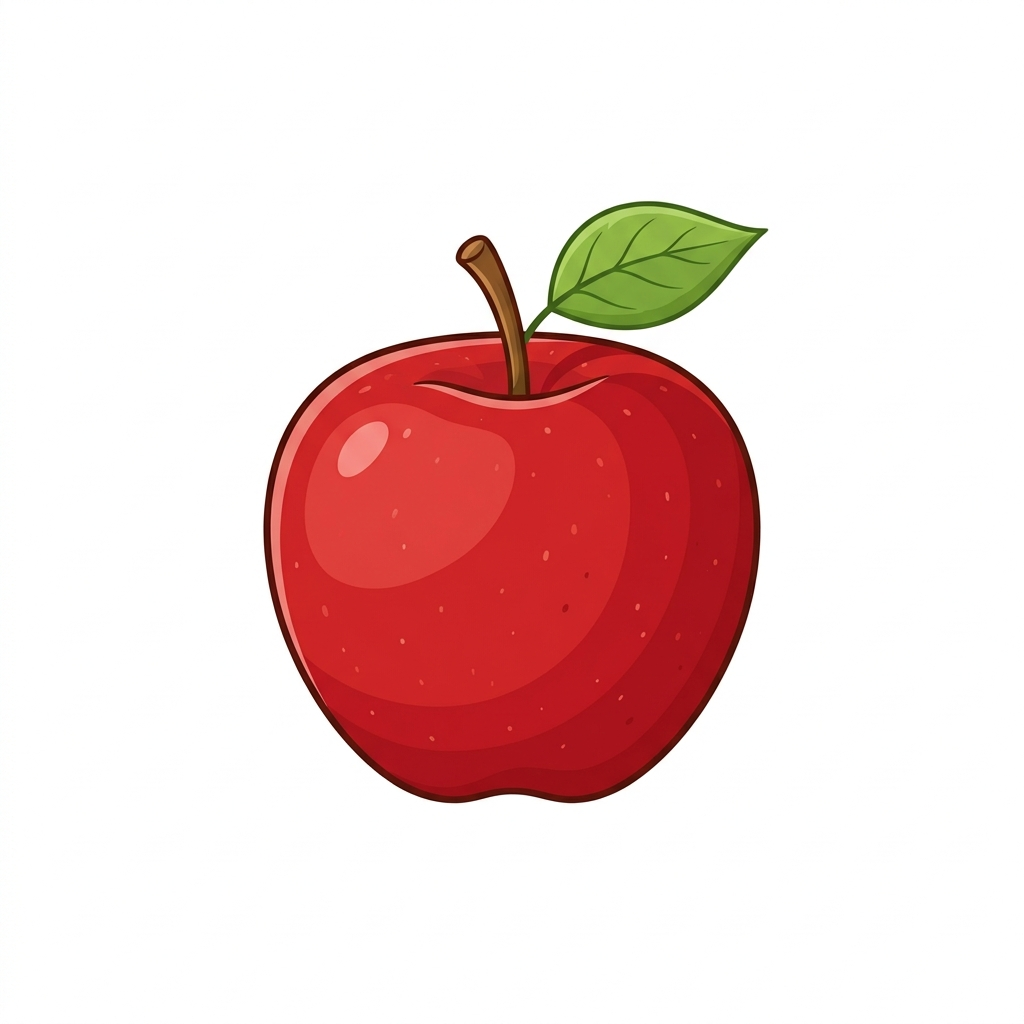
\includegraphics[width=0.9\linewidth]{vokab_300dpi/apel.png} \\
            \small\textit{Den Apel (La pomme / The apple)}
            \vspace{0.5cm}
        }}
    \end{minipage}
    \hfill
    \begin{minipage}[t]{0.48\textwidth}
        \centering
        \textbf{Eng Banann}
        \vspace{0.5em}
        \framebox{\parbox{0.9\linewidth}{\centering
            \vspace{0.5cm}
            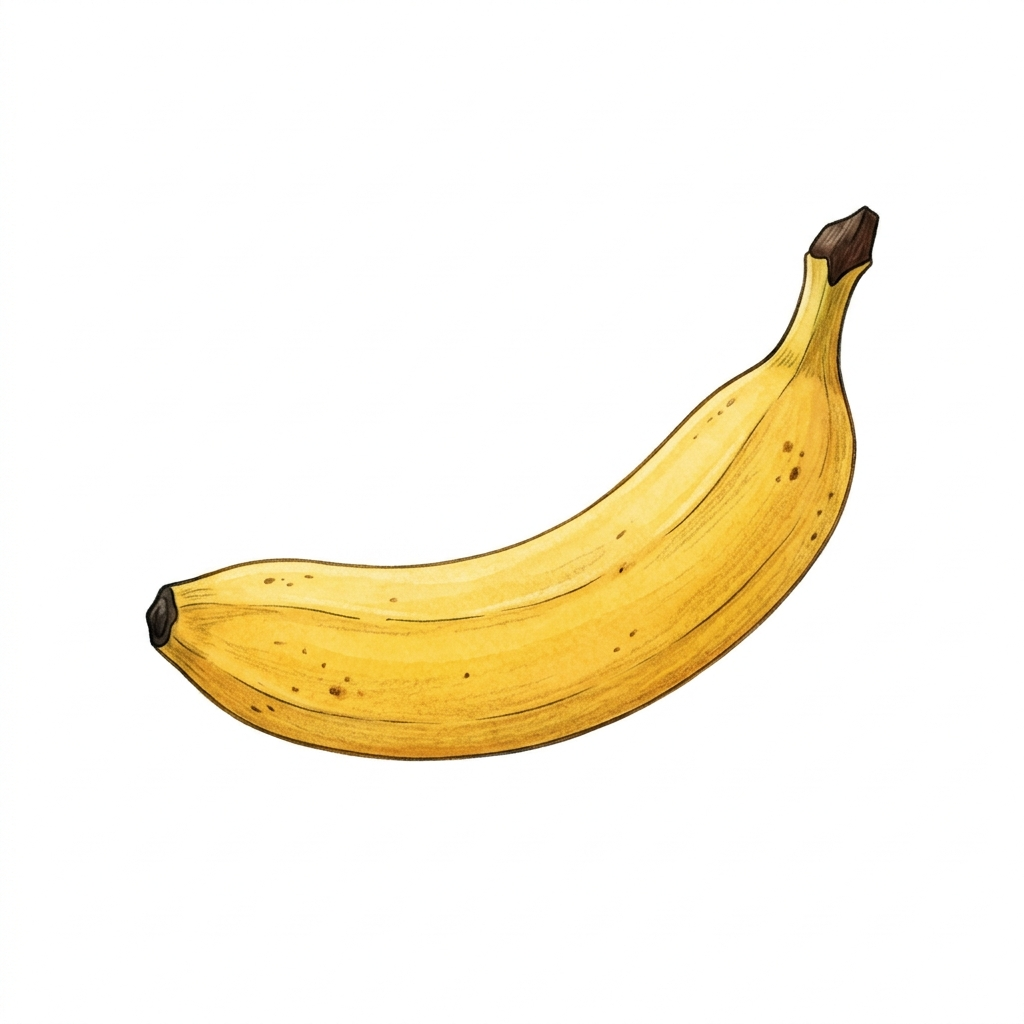
\includegraphics[width=0.9\linewidth]{vokab_300dpi/banann.png} \\
            \small\textit{Eng Banann (La banane / The banana)}
            \vspace{0.5cm}
        }}
    \end{minipage}
    
    \vspace{1.5em}
    
    \begin{minipage}[t]{0.48\textwidth}
        \centering
        \textbf{D'Zopp}
        \vspace{0.5em}
        \framebox{\parbox{0.9\linewidth}{\centering
            \vspace{0.5cm}
            
\includegraphics[width=0.9\linewidth]{vokab_300dpi/zopp.png} \\
            \small\textit{D'Zopp (La soupe / The soup)}
            \vspace{0.5cm}
        }}
    \end{minipage}
    \hfill
    \begin{minipage}[t]{0.48\textwidth}
        \centering
        \textbf{De / D'Garage}
        \vspace{0.5em}
        \framebox{\parbox{0.9\linewidth}{\centering
            \vspace{0.5cm}
            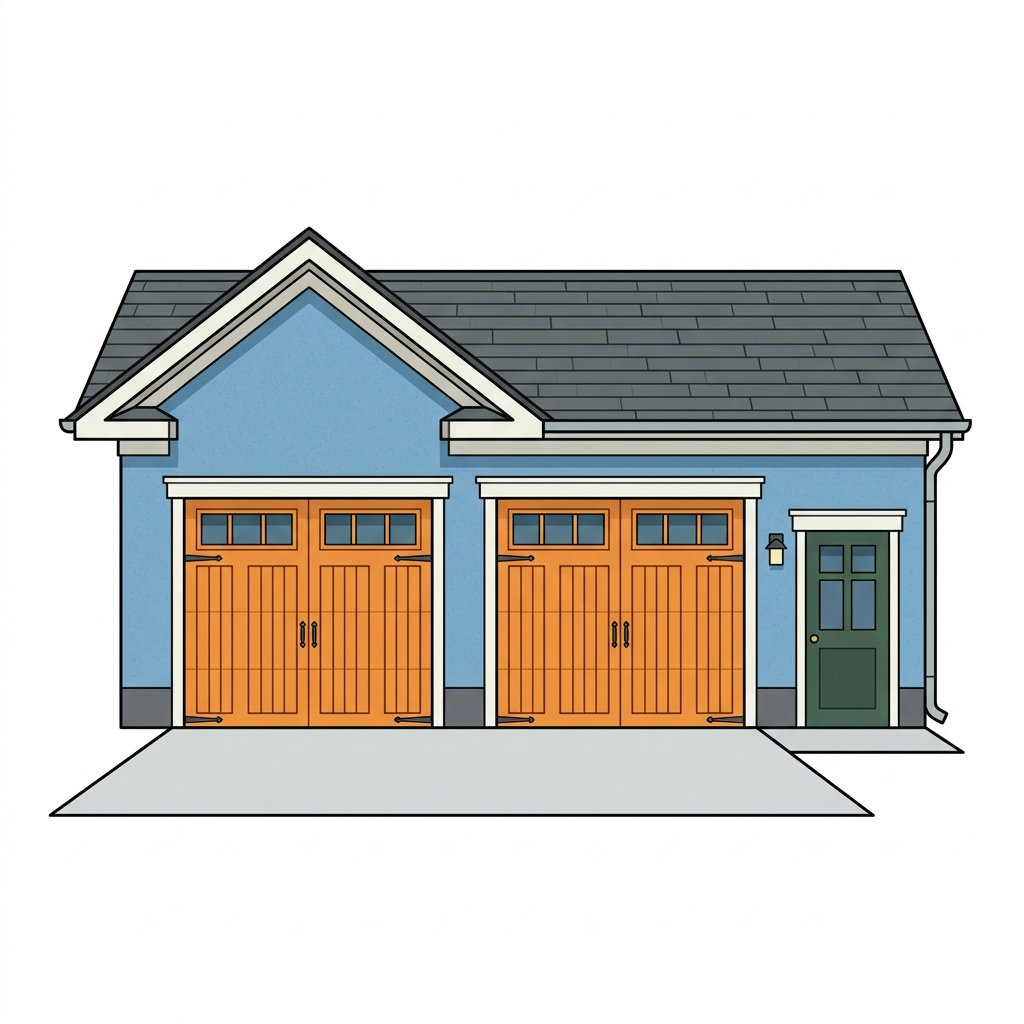
\includegraphics[width=0.9\linewidth]{vokab_300dpi/garage.png} \\
            \small\textit{De / D'Garage (Le garage / The garage)}
            \vspace{0.5cm}
        }}
    \end{minipage}
    
    \vspace{1.5em}
    
    \begin{minipage}[t]{0.48\textwidth}
        \centering
        \textbf{Den Hënneschten}
        \vspace{0.5em}
        \framebox{\parbox{0.9\linewidth}{\centering
            \vspace{0.5cm}
            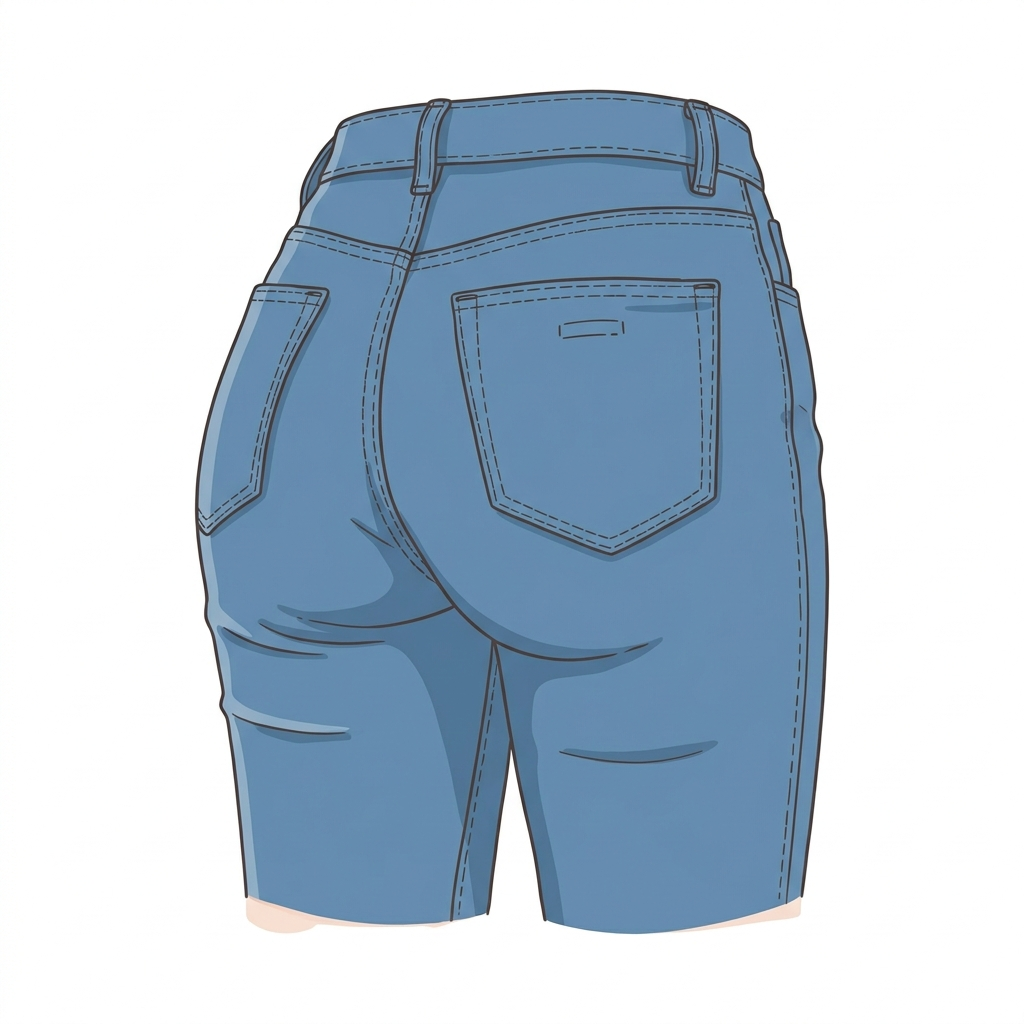
\includegraphics[width=0.9\linewidth]{vokab_300dpi/henneschten.png} \\
            \small\textit{Den Hënneschten (Le derrière / The bottom)}
            \vspace{0.5cm}
        }}
    \end{minipage}
\end{center}
